\documentclass[mathserif]{beamer}

\usepackage{subg}
\usepackage{pdfpages}

\title[Discrete Sampling using Semigradient-based Product Mixtures]
{Discrete Sampling using Semigradient-based Product Mixtures}

\author[Alkis Gotovos]{}

\begin{document}

\setbeamertemplate{background canvas}{}
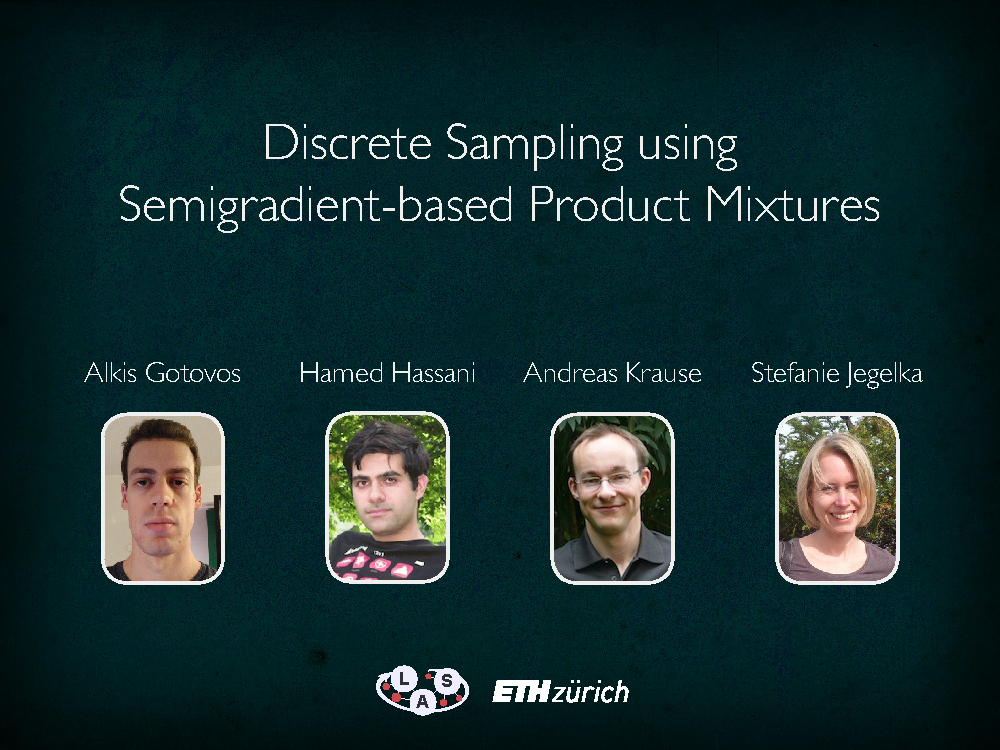
\includepdf[pages={1}]{title/title.pdf}
\setbeamertemplate{background canvas}{
\includegraphics[width=\paperwidth]{figures/bg_no_line.png}}


\begin{frame}{Modeling gene alterations}
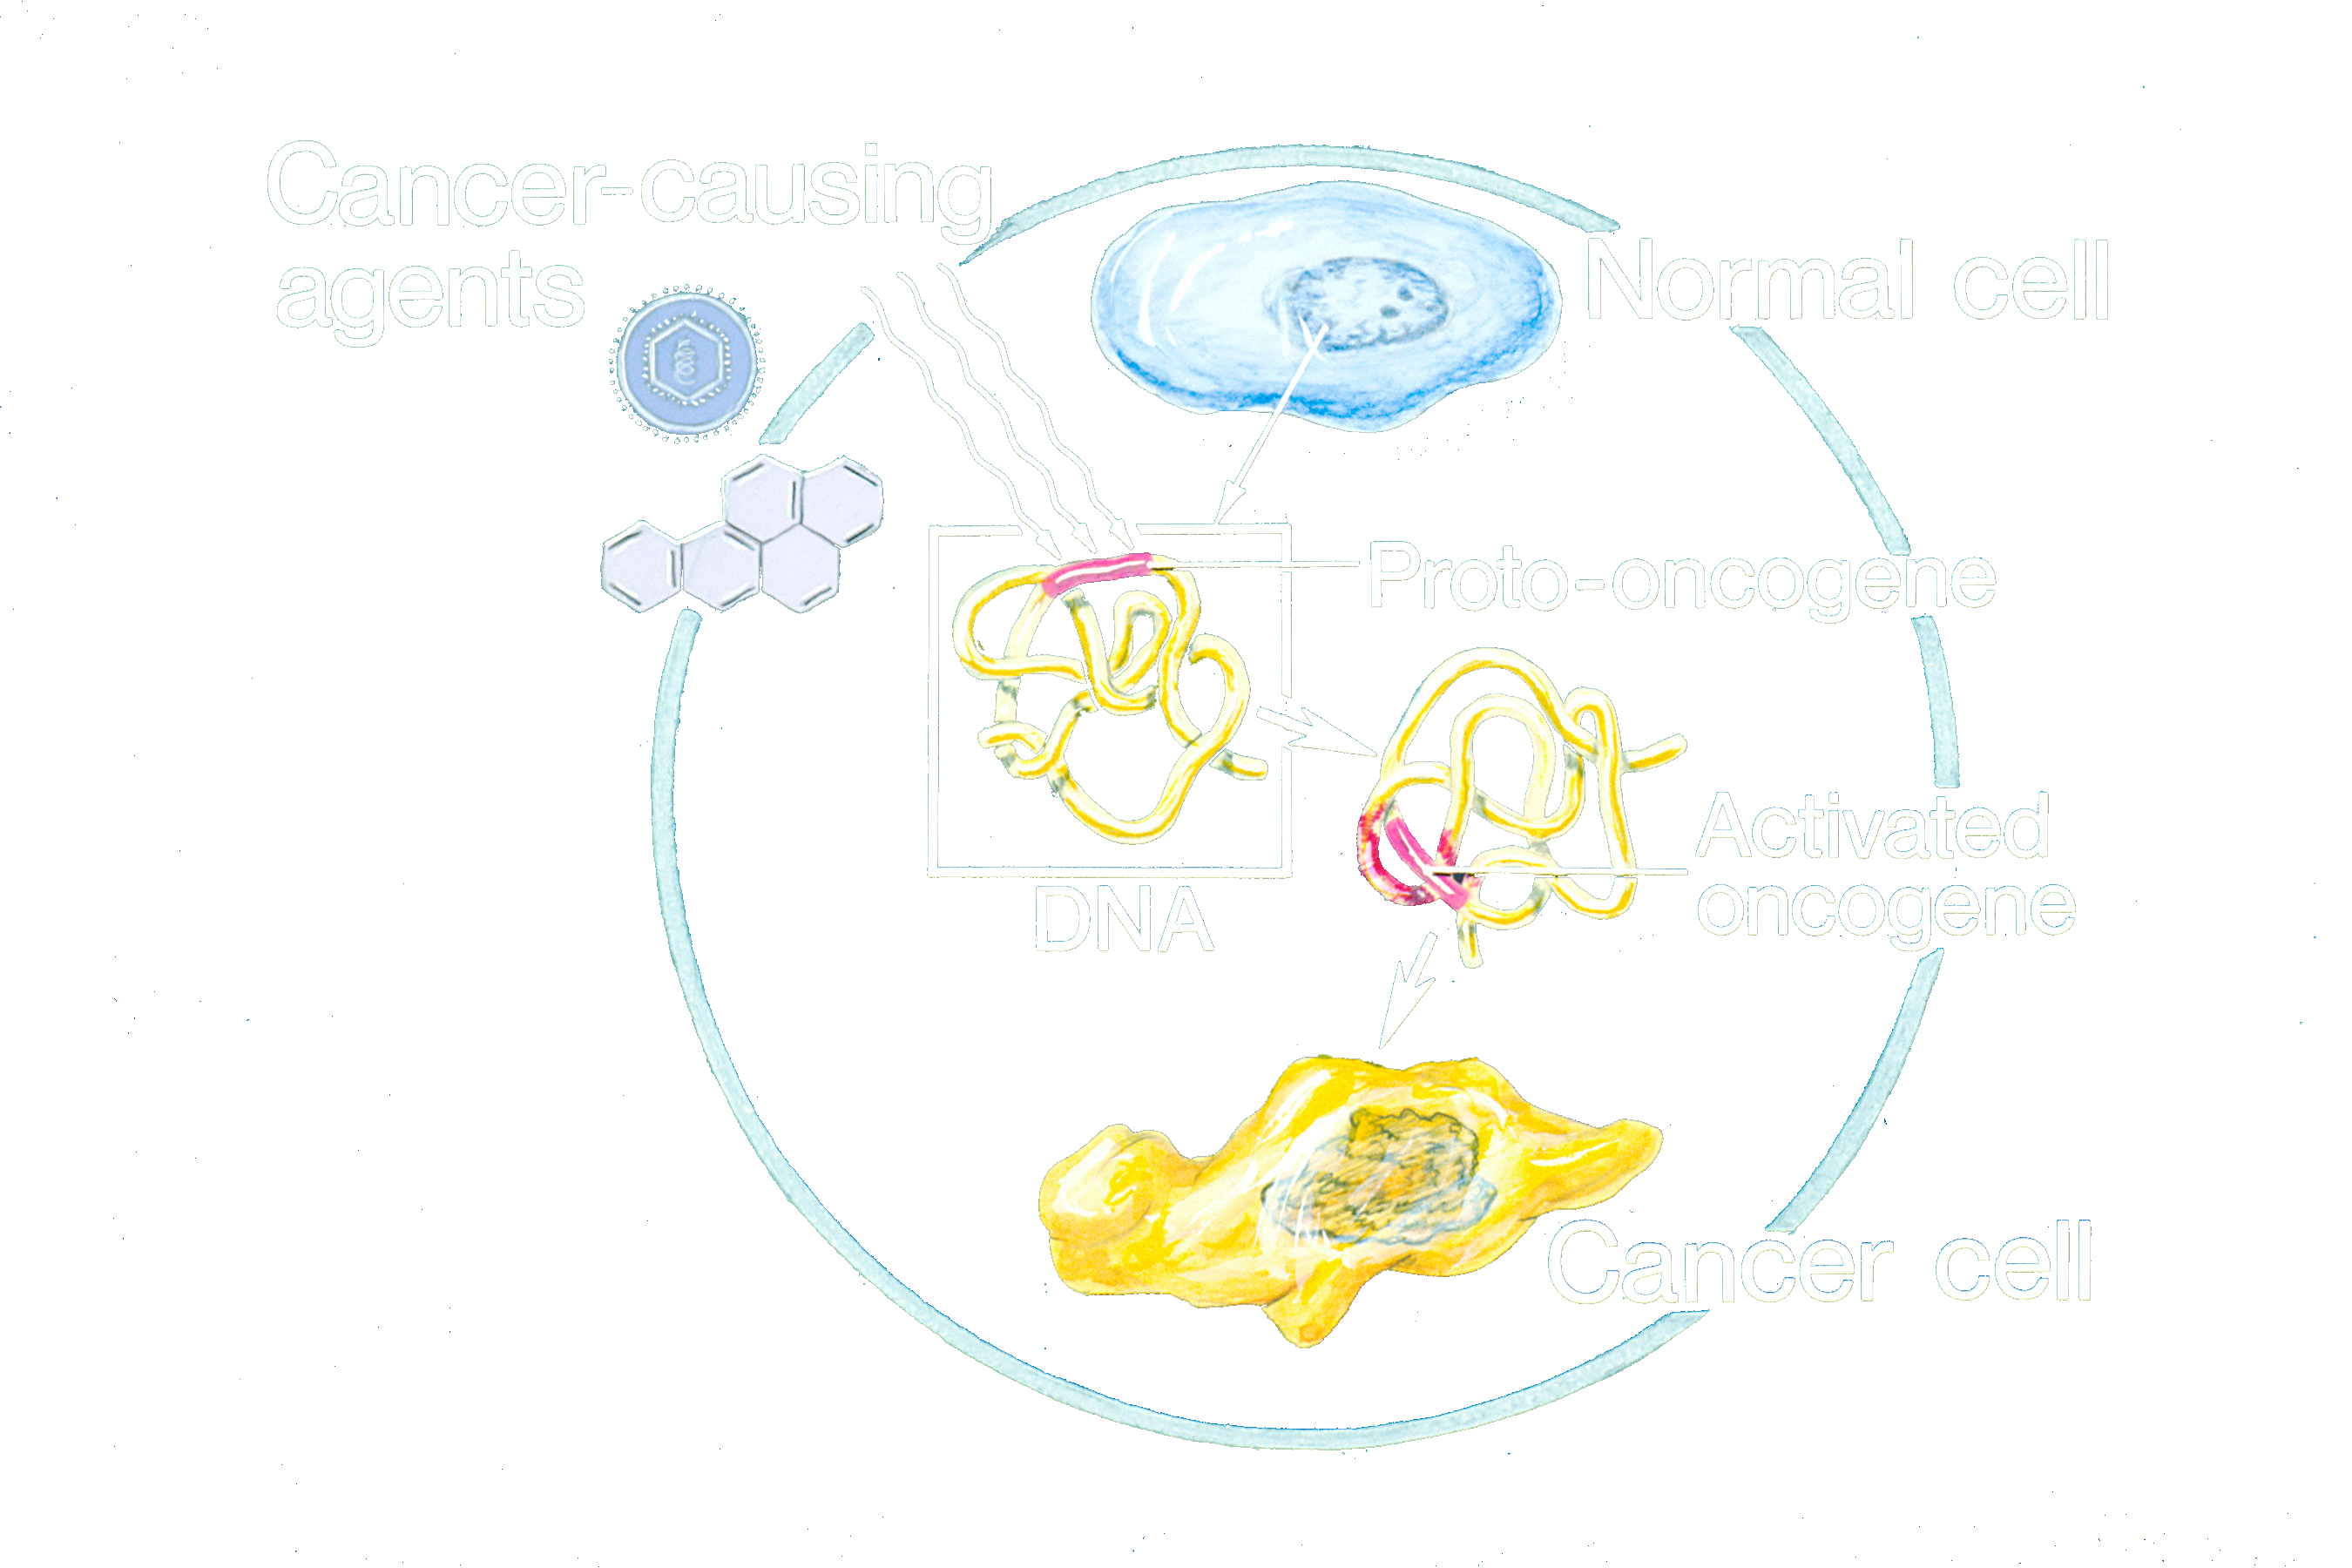
\includegraphics[width=3.7in]{figures/oncogene.png}\\
\qsource{\texttt{cancergenome.nih.gov}}
\end{frame}


\begin{frame}{Modeling gene alterations}
\centering
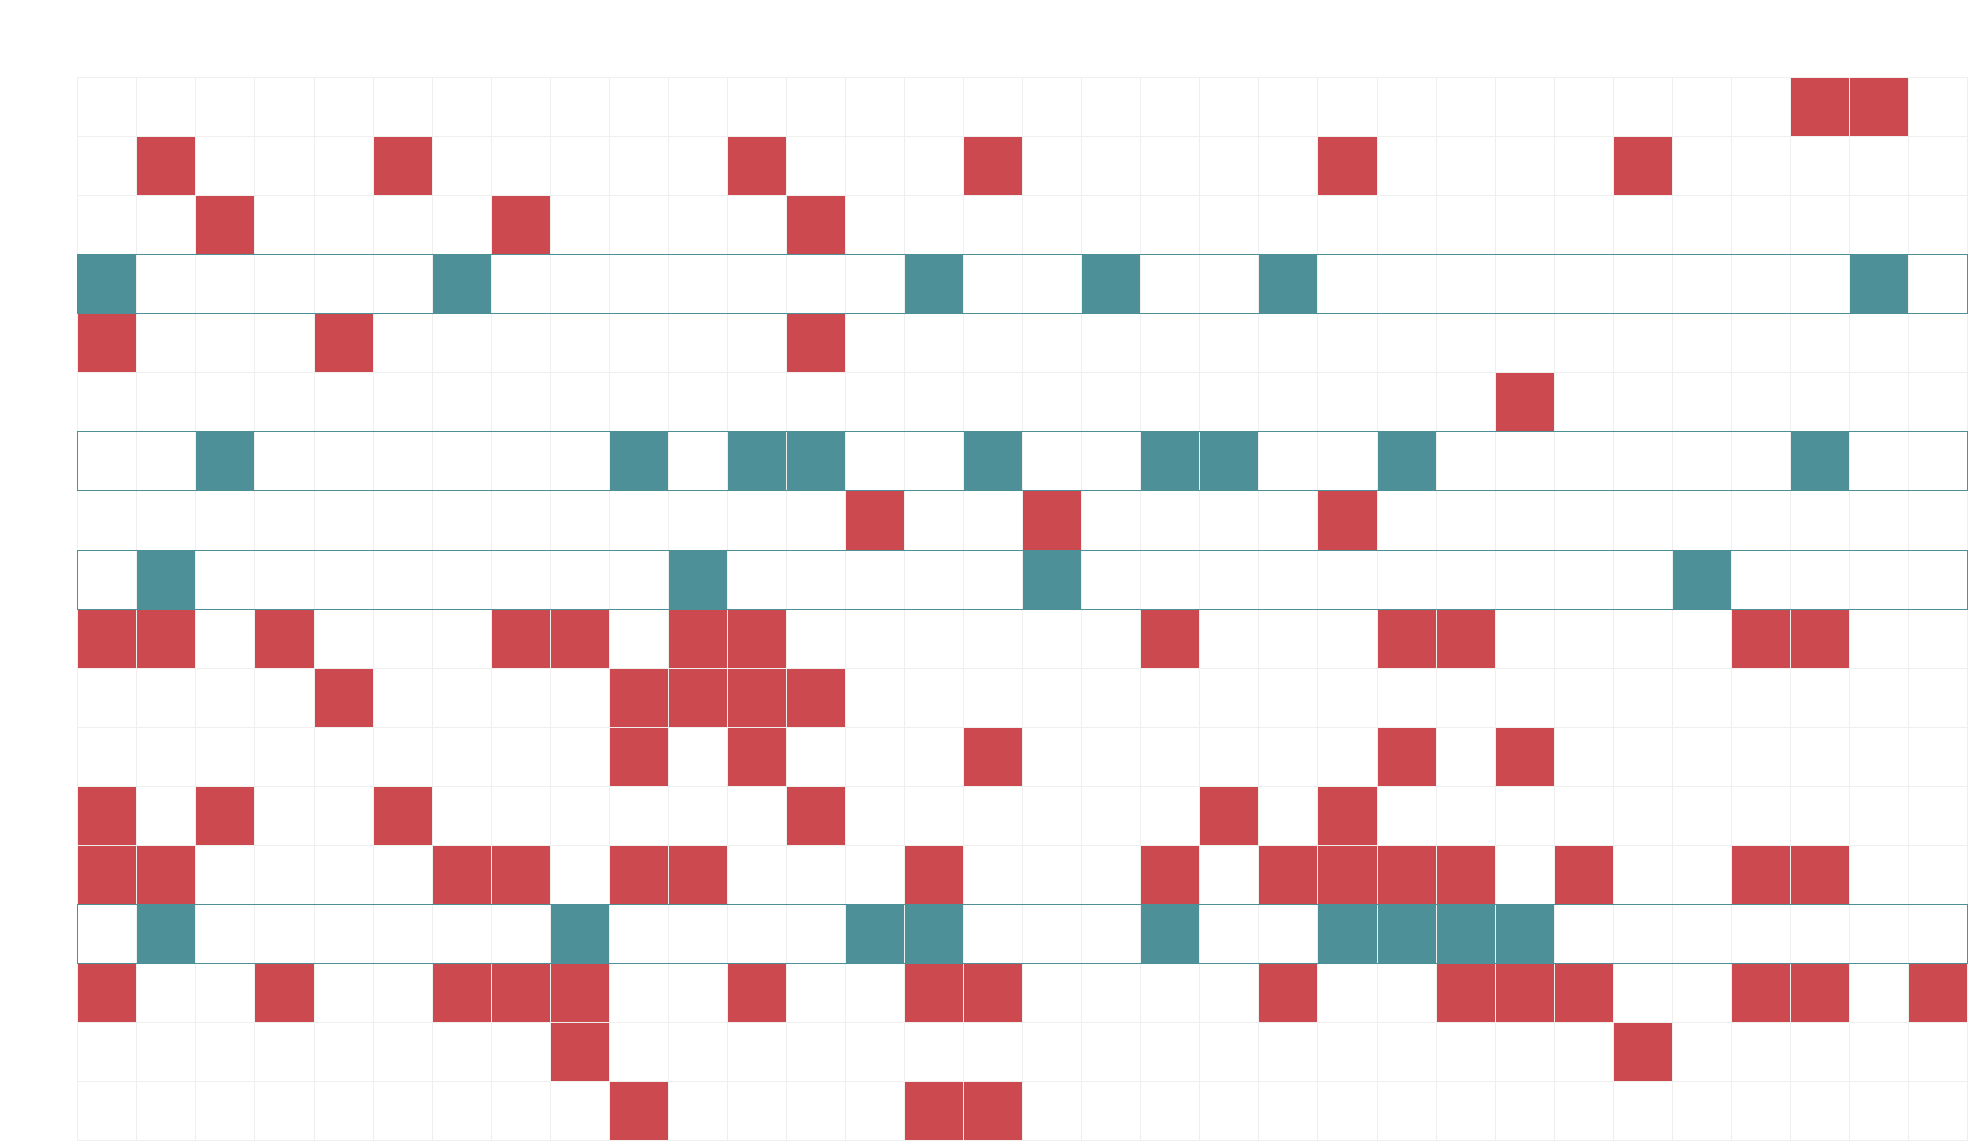
\includegraphics[width=\textwidth]{figures/grid_genes.pdf}
\end{frame}


\begin{frame}{Modeling gene alterations}
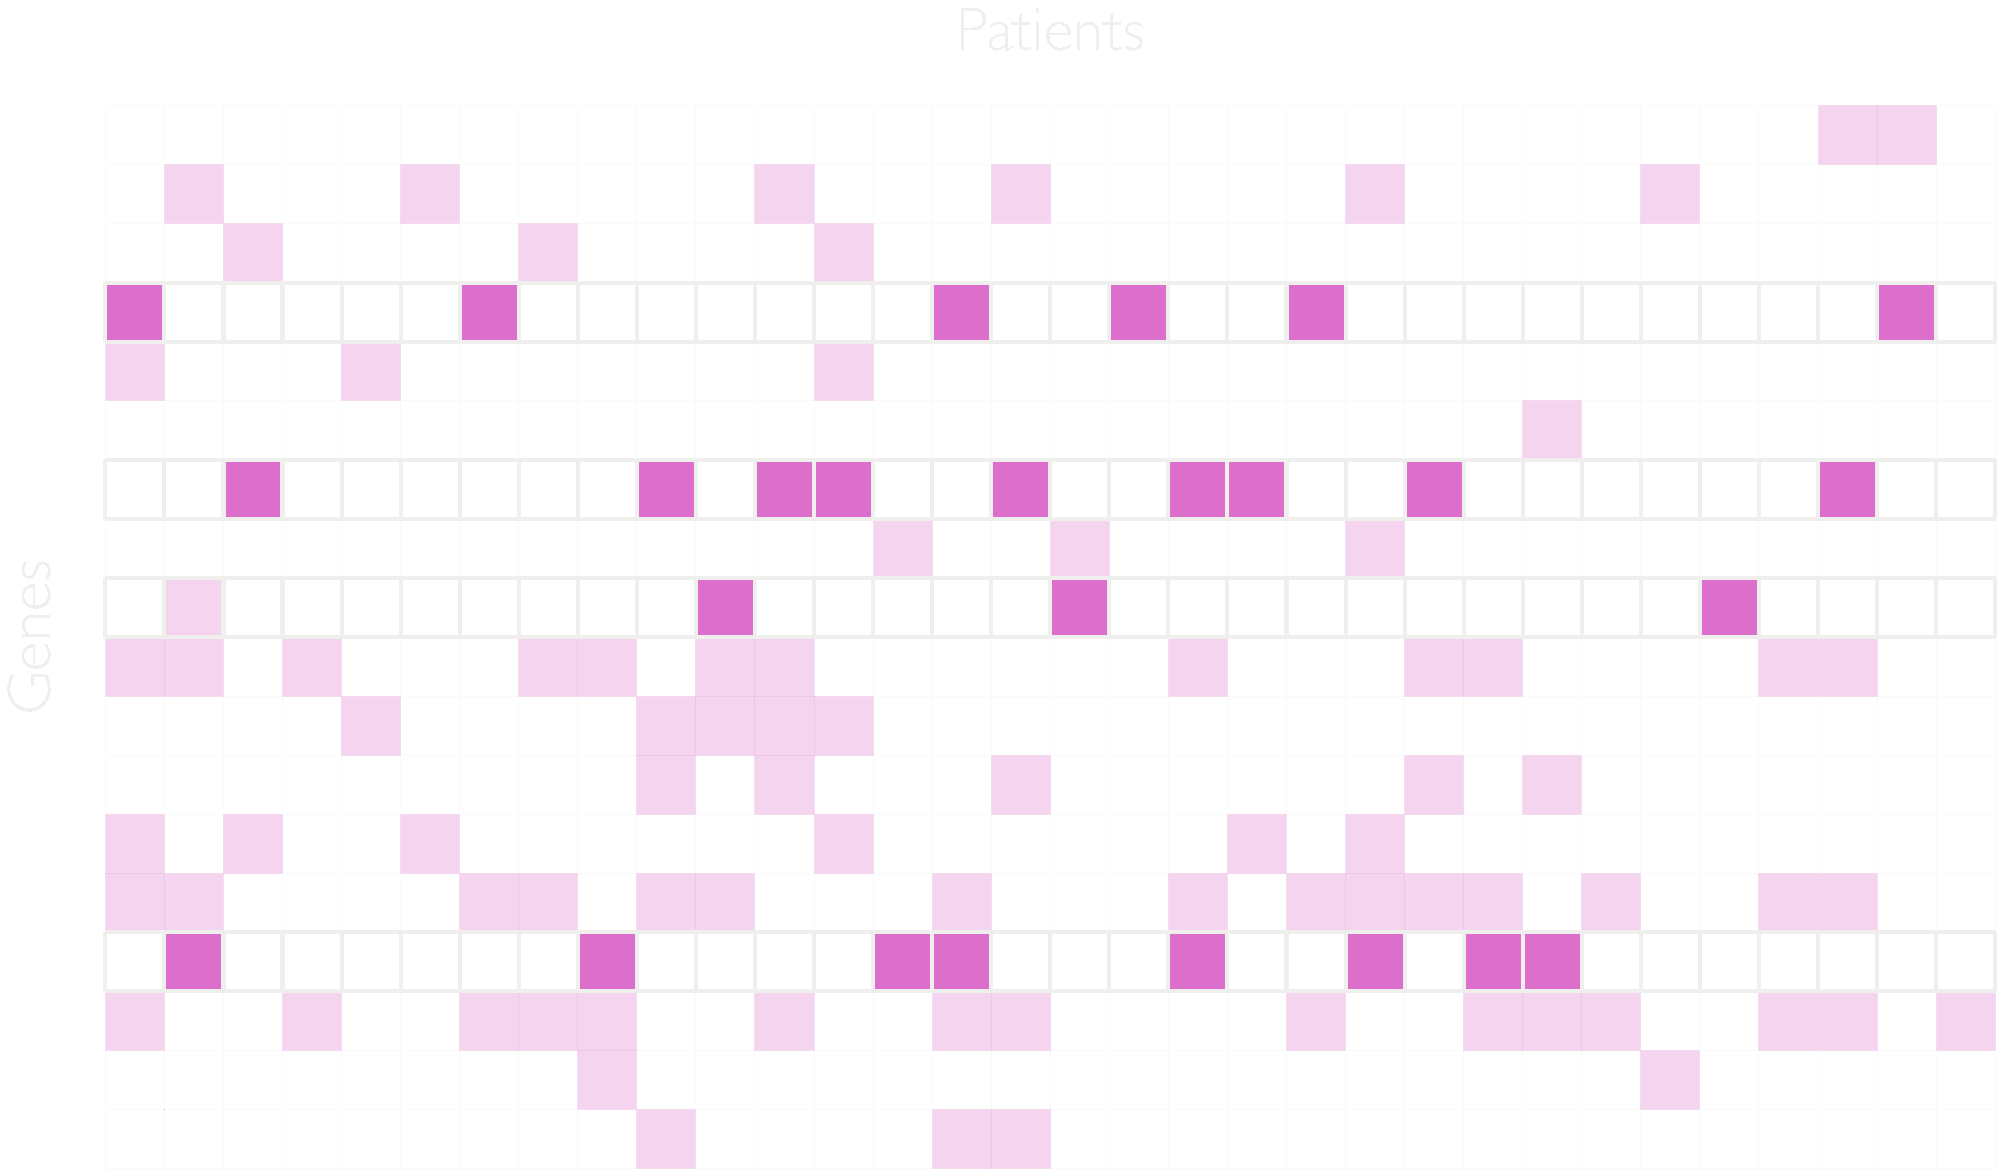
\includegraphics[width=\textwidth]{figures/grid_genes_muex.pdf}
\end{frame}


\begin{frame}{Modeling gene alterations}
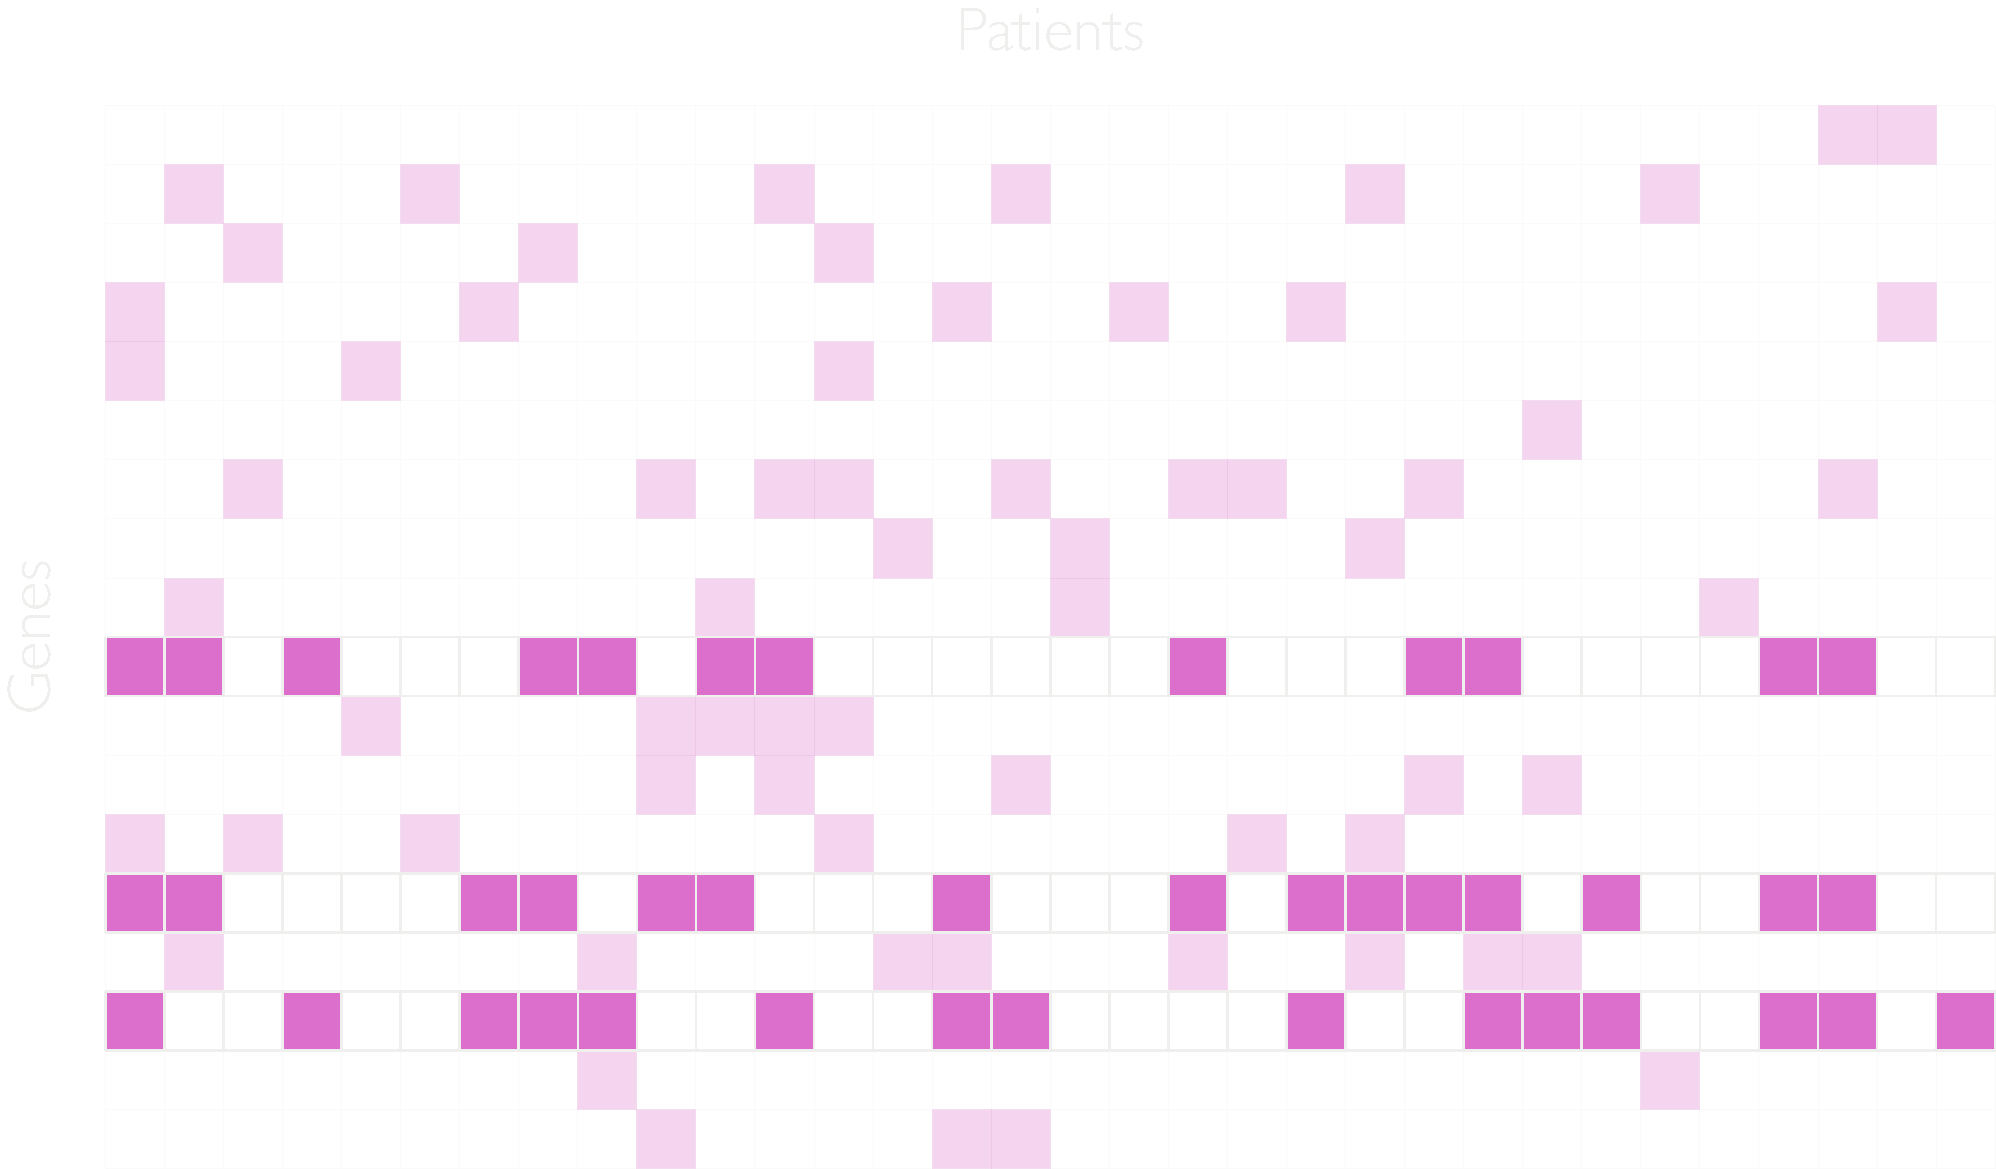
\includegraphics[width=\textwidth]{figures/grid_genes_cooc.pdf}
\end{frame}


\begin{frame}{Modeling teams in online games}
\vspace{1em}
\centering

\includegraphics[width=3.5in]{figures/openai_dota.png}\\
\qsource{\texttt{www.theverge.com}}
\end{frame}


\begin{frame}{Modeling teams in online games}
\vspace{1em}
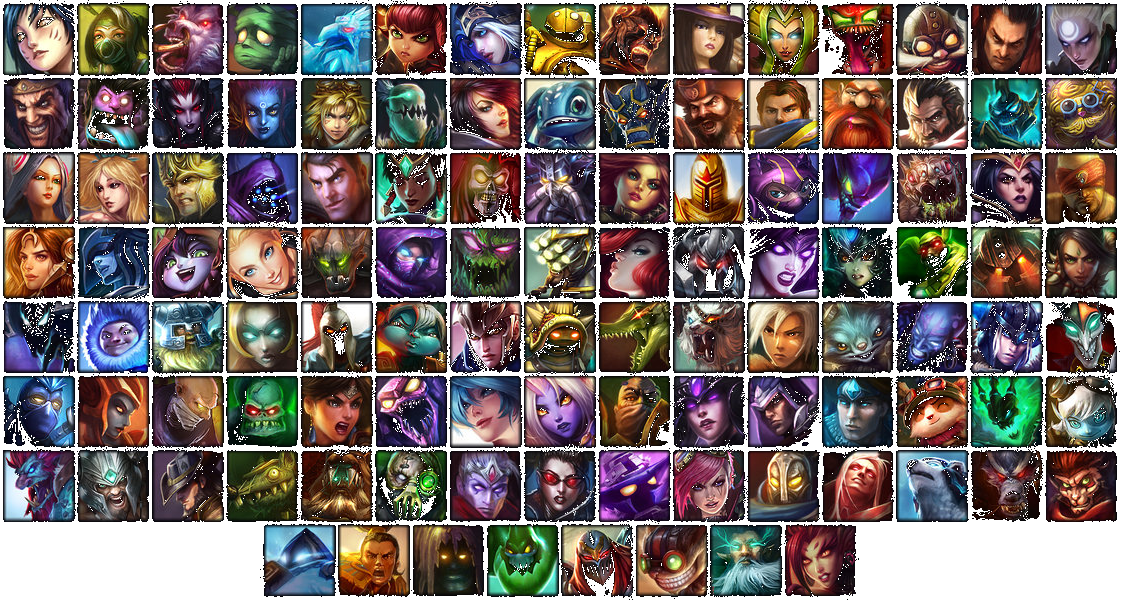
\includegraphics[width=\textwidth]{figures/lol_champs.png}\\
\qsource{\texttt{euw.leagueoflegends.com}}
\end{frame}


\begin{frame}{Modeling teams in online games}
\centering
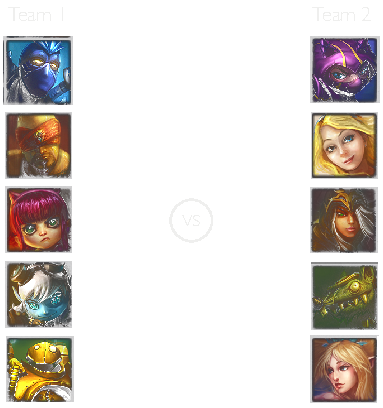
\includegraphics[height=2.7in]{figures/champions5v5.pdf}
\end{frame}


\begin{frame}{Modeling teams in online games}
\centering
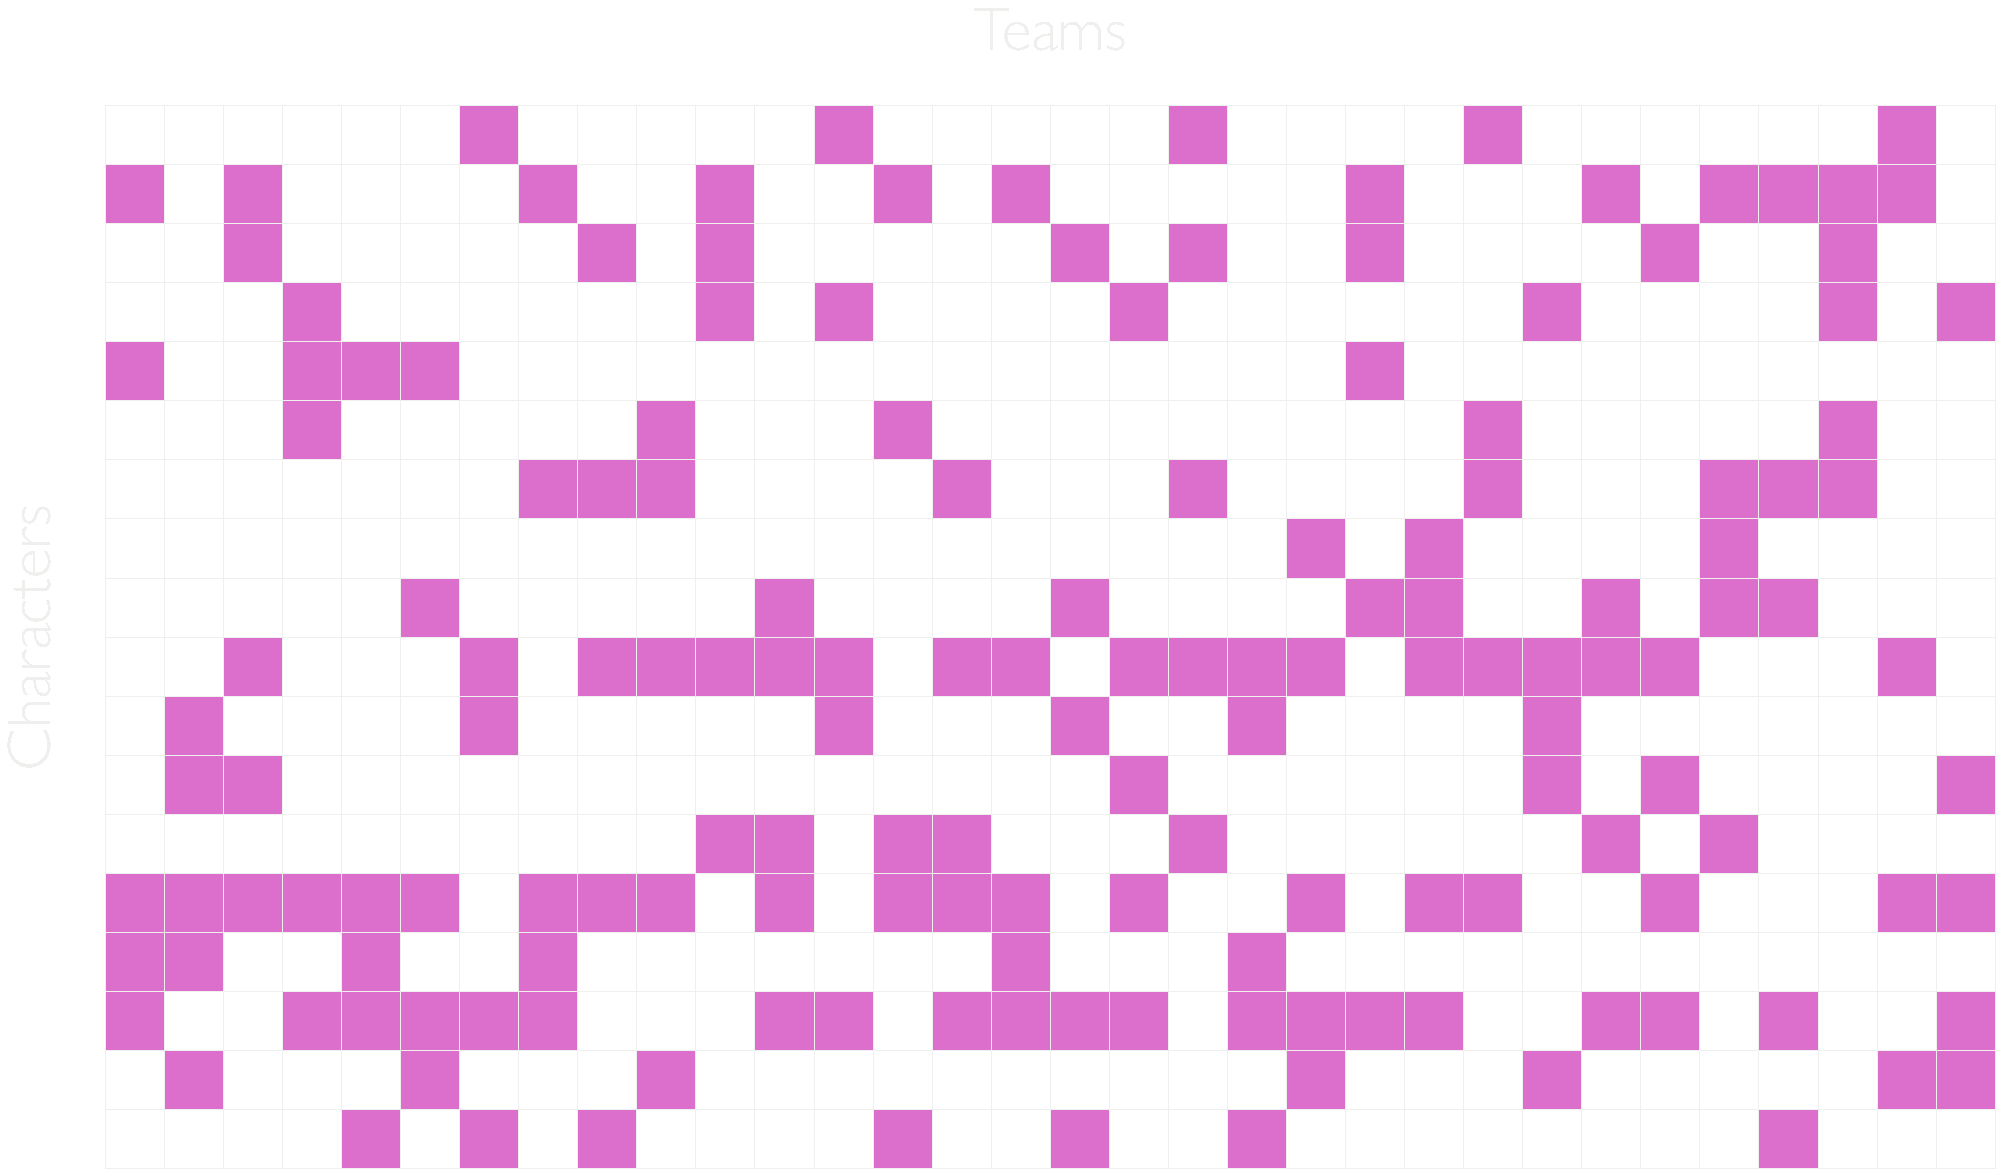
\includegraphics[width=\textwidth]{figures/grid_hots.pdf}
\end{frame}


\begin{frame}{Discrete probabilistic models}
\vspace{0.7em}
\begin{columns}[t]
\begin{column}{0.5\textwidth}
\uncover<1->{%
\centering
Ground set\\[0.2em]
$V = \{1,\ldots,n\}$

\vspace{1em}
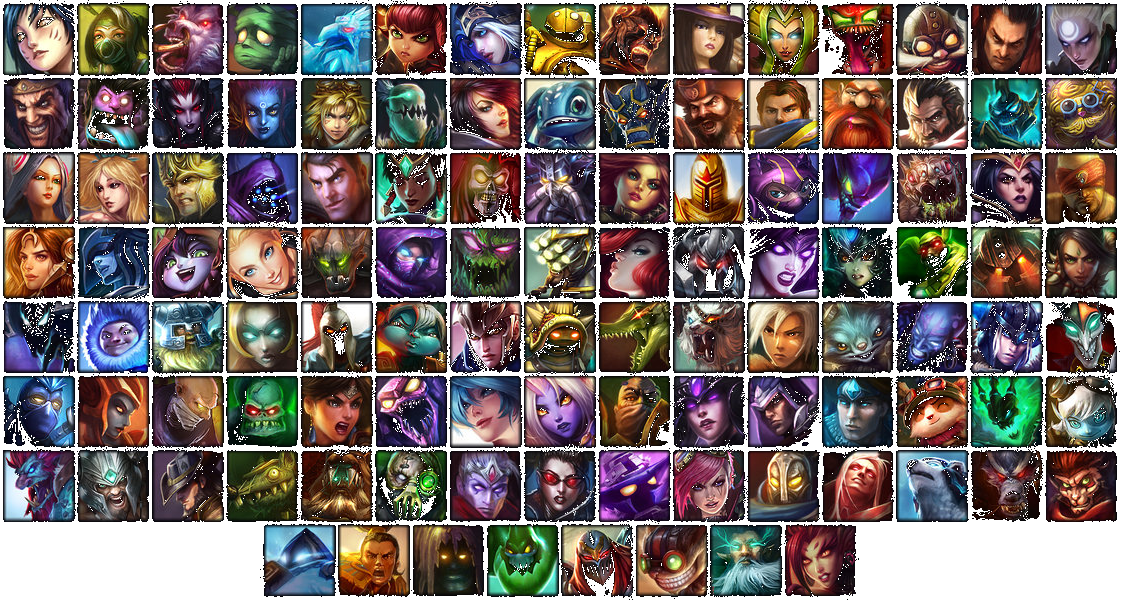
\includegraphics[width=1.5in]{figures/lol_champs.png}%
}
\end{column}
\begin{column}{0.5\textwidth}
\uncover<2->{%
\centering
Data\\[0.2em]
$\mathcal D = \{S_i\}_{i=0}^m$, $S_i \subseteq V$

\vspace{0.5em}
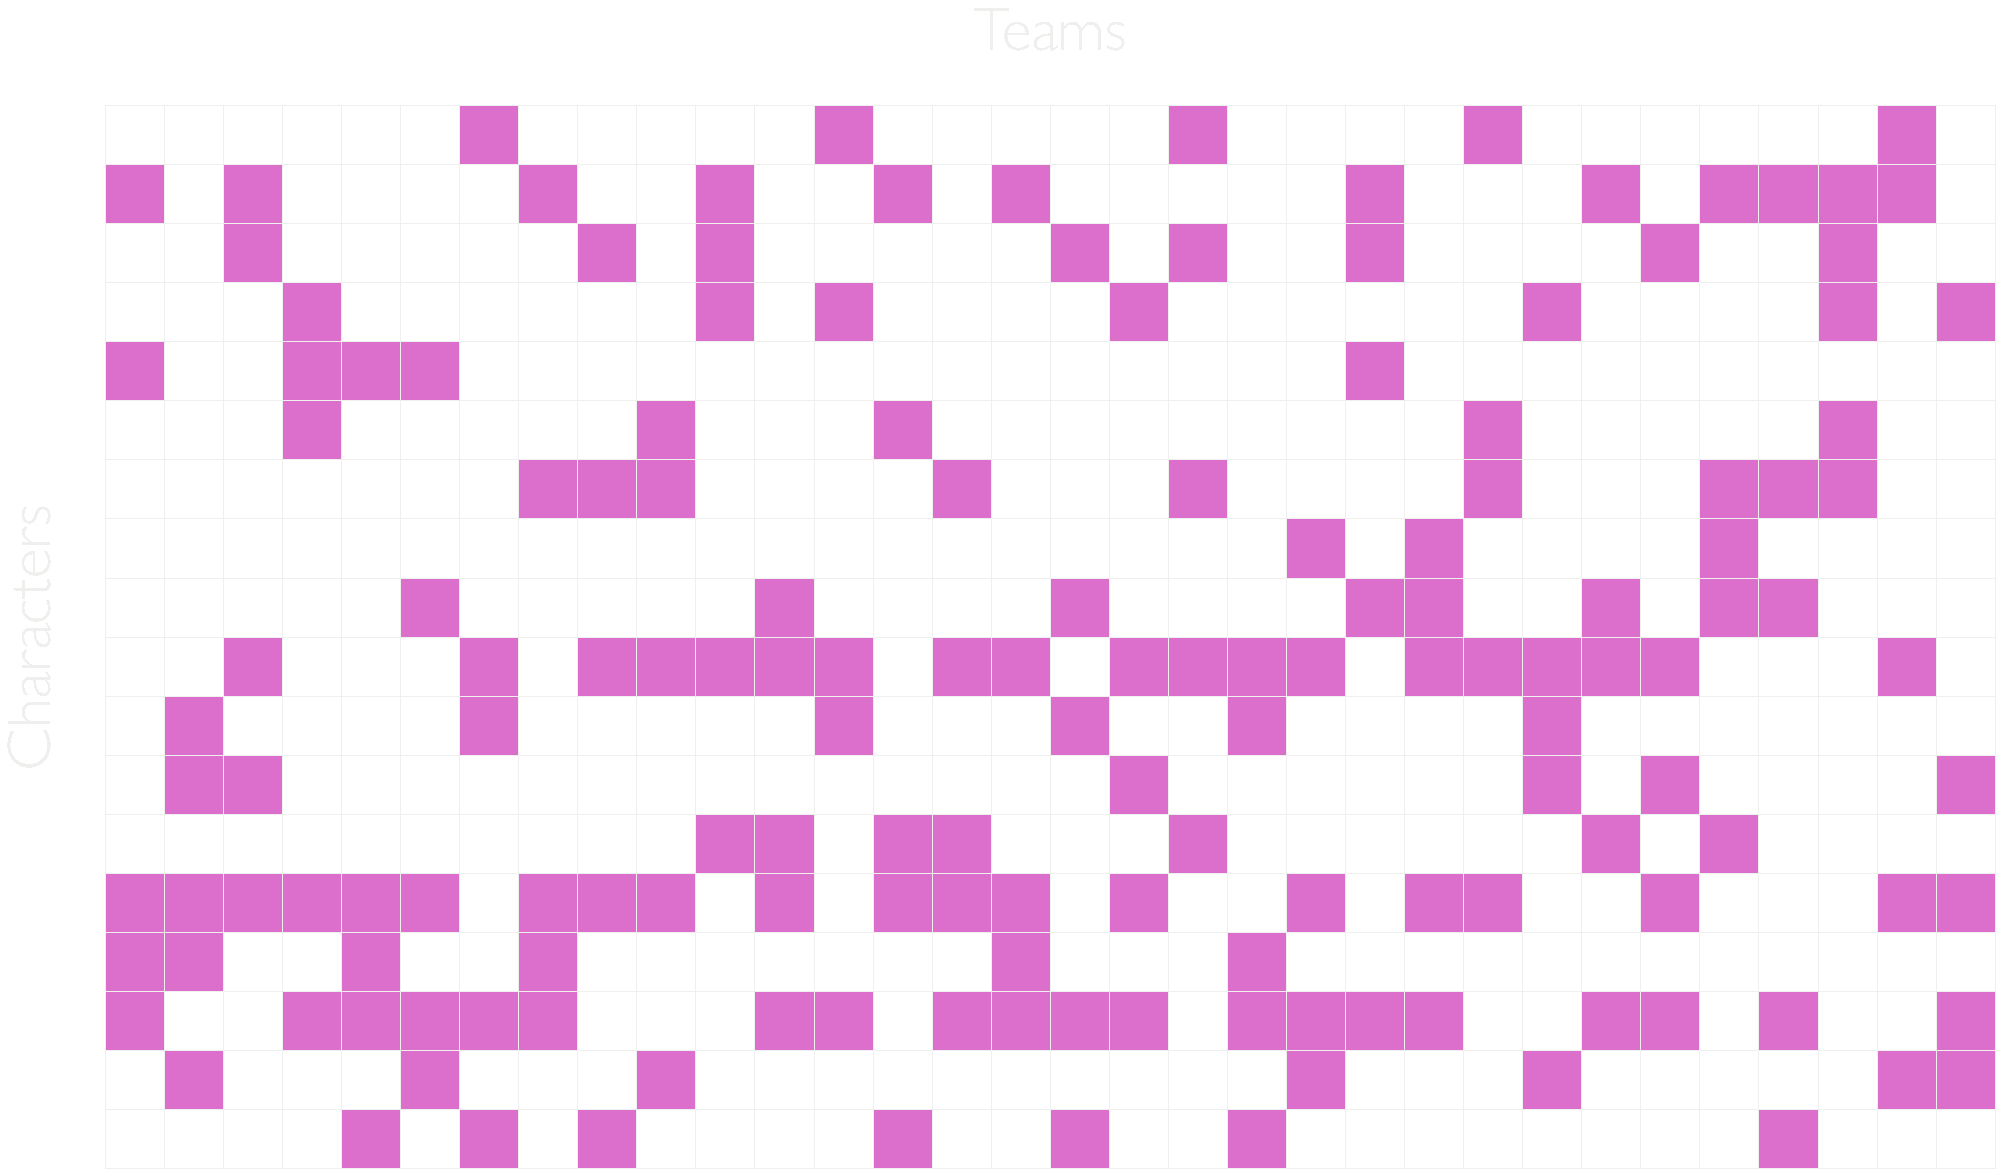
\includegraphics[width=1.4in]{figures/grid_hots.pdf}%
}
\end{column}
\end{columns}

\vspace{1.5em}

\begin{center}
\uncover<3->{%
Model {\color{col2}higher-order} interactions\\[0.3em]

\qboxb{
$p(S; \theta) = \displaystyle\frac{1}{Z(\theta)}\exp \big( F(S; \theta) \big)$
}%
}
\vspace{0.6em}

\begin{minipage}{0.49\textwidth}
\footnotesize
\begin{itemize}
\item<4-> $F(S) = \textrm{graph-cut}(S)\ \rightarrow\ $ Ising model
\item<5-> $F(S) = \log \left|K_S\right|\ \rightarrow\ $ DPP
\end{itemize}
\end{minipage}

\end{center}

\end{frame}


\begin{frame}{Discrete probabilistic models}
\centering
\begin{tikzpicture}[
box/.style={minimum height=4em}
]
  \node[box,text=textcolor] (1) at (0,0) {Learn $\theta$};
  \uncover<2->{
  \node[box,text=textcolor,anchor=west] (12) at (0.3,-1.5) {Max. likelihood};
  }
  \only<3,4>{
  \node[box,text=textcolor] (2) at (0,-3) {Compute $\nabla_{\theta}Z(\theta)$};
  }
  \only<3->{
  \draw [-latex, color=textcolor, line width=0.5] (2) to (1);
  }
  \uncover<4->{
  \node[box,text=textcolor,anchor=west] (23) at (0.3,-4.5) {\#P-hard in general};
  }
  \uncover<5->{
  \node[box, text=textcolor] (2) at (0,-3) {{\color{col2}Approximate} \color{textcolor}$\nabla_{\theta}Z(\theta)$};
  \only<1-5>{
  \node[box, text=textcolor] (3) at (0,-6) {Sample from $p(\cdot\,; \theta)$};
  \draw [-latex, color=textcolor, line width=0.5] (3) to (2);
  }
  \only<6->{
  \node[box, text=textcolor] (3) at (0,-6) {\qboxb{Sample from $p(\cdot\,; \theta)$}};
  \draw [-latex, color=textcolor, line width=0.5] (3) to (2);
  }
  }
\end{tikzpicture}
\end{frame}


\begin{frame}{The Gibbs sampler}
\centering
\only<1>{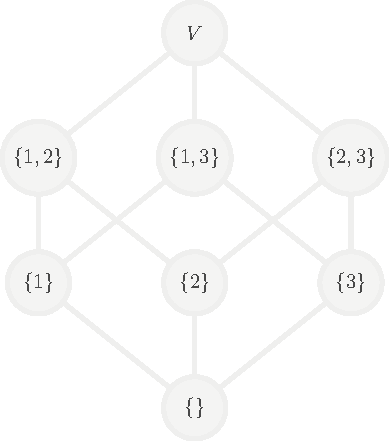
\includegraphics[width=2.5in]{figures/lattice_full.pdf}}%
\only<2>{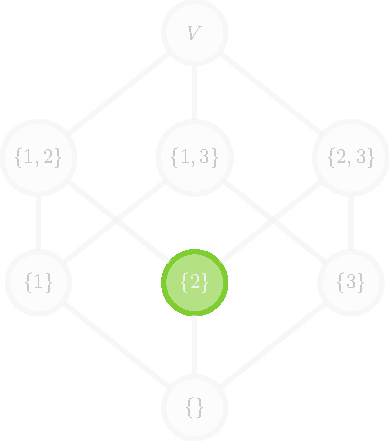
\includegraphics[width=2.5in]{figures/lattice_gibbs_1.pdf}}%
\only<3>{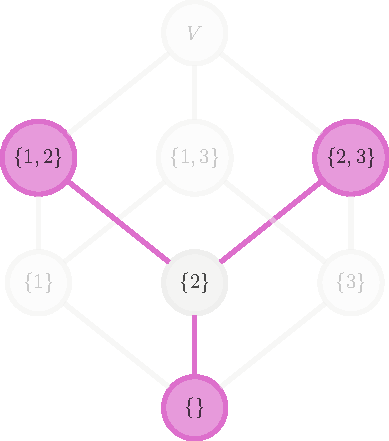
\includegraphics[width=2.5in]{figures/lattice_gibbs_2.pdf}}
\end{frame}


\begin{frame}{When Gibbs fails}
\centering
\only<1>{
\includegraphics[width=\textwidth]{figures/bottleneck0.pdf}}%
\only<2>{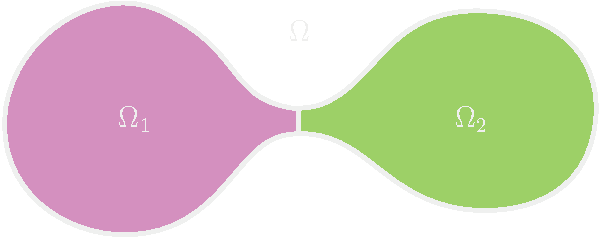
\includegraphics[width=\textwidth]{figures/bottleneck1.pdf}}%
\only<3>{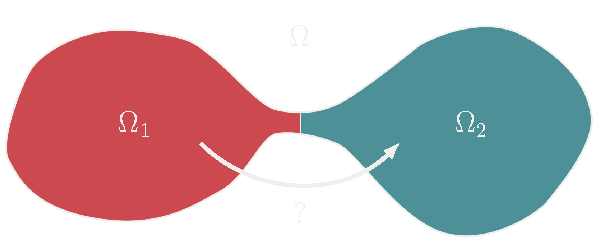
\includegraphics[width=\textwidth]{figures/bottleneck2.pdf}}
\end{frame}


\begin{frame}{The $\mathrm{M}^3$ chain}
\vspace{0.8em}
$\rightarrow\ \ $$\mathrm{M}^3$ = Mixture of Log-Modulars Metropolis

\vspace{-1em}
\uncover<2->{
\renewcommand{\arraystretch}{1}
\begin{tabular}{>{\arraybackslash}p{0.28\textwidth}>{\arraybackslash}p{0.71\textwidth}}

\begin{minipage}[t]{\textwidth}
\vspace{1.8em}
\only<7-8>{\color{col2}} \circled{1}\hspace{0.3em} Mixture
\end{minipage}
&
\begin{minipage}[t]{\textwidth}
\uncover<8->{%
\vspace{1em}
\only<1-10>{$q(S, T) = \displaystyle\frac{1}{Z_q} \sum_{i = 1}^{r} w_i\exp\left(m_i(T) \right)$}%
\only<11->{${\color{col2}q(T)} = \displaystyle\frac{1}{Z_q} \sum_{i = 1}^{r} w_i\exp\left(m_i(T) \right)$}
\vspace{1em}%
}
\end{minipage}\\ \midrule

\begin{minipage}[t]{\textwidth}
\vspace{1.15em}
\only<9-10>{\color{col2}} \circled{2}\hspace{0.3em} Log-Modulars
\end{minipage}
&
\begin{minipage}[t]{\textwidth}
\uncover<10->{
\vspace{1em}
$m_i(T) = \displaystyle\sum_{v \in T} m_{iv}$
\vspace{1em}
}
\end{minipage}\\ \midrule

\begin{minipage}[t]{\textwidth}
\vspace{2.45em}
\only<3-6>{\color{col2}} \circled{3}\hspace{0.3em} Metropolis
\end{minipage}
&
\begin{minipage}[t]{\textwidth}
\vspace{1em}
\begin{itemize}
\item<4-> Target $\ p(S) \propto \exp(F(S))$
\vspace{0.15em}
\item<5-> \only<5-10>{Proposal $\ q(S, T)$}%
\only<11->{Proposal \color{col2} $\ q(T)$}%
\item<6-> Accept with probability%
\only<6-10>{$\ \min\left\{1, \frac{p(T)q(T, S)}{p(S)q(S, T)}\right\}$}%
\only<11->{$\ \min\left\{1, \frac{p(T)\color{col2}q(S)}{p(S)\color{col2}q(T)}\right\}$}%
\end{itemize}
\vspace{1em}
\end{minipage}

\end{tabular}
}
\end{frame}


\begin{frame}{The $\mathrm{M}^3$ chain}
\vspace{0.5em}
Proposal$\ \ \ q(T) = \displaystyle\frac{1}{Z_q} \sum_{i = 1}^{r} w_i\exp\left(m_i(T) \right)$

\vspace{2em}
\uncover<2->{%
$\rightarrow\ \ $ Can sample from $q$ in $\mathcal{O}(n + r)$ time
}
\uncover<3->{%
\vspace{2em}
\qprop{1}{Mixture $q$ can approximate any distribution $p$ arbitrarily well.}
\vspace{-0.7em}
}
\uncover<4->{%
\begin{center}
{\color{col1}BUT}

\vspace{0.5em}
{\color{col1}May need an exponential (in $n$) number of components $r$}
\end{center}
}
\end{frame}


\begin{frame}{The combined chain}
\vspace{0.5em}
Gibbs step with probability $\alpha$ \hspace{1em}|\hspace{1em} $\mathrm{M}^3$ step with prob. $1 - \alpha$

\uncover<2->{%
\vspace{2em}
\centering
\only<1-2>{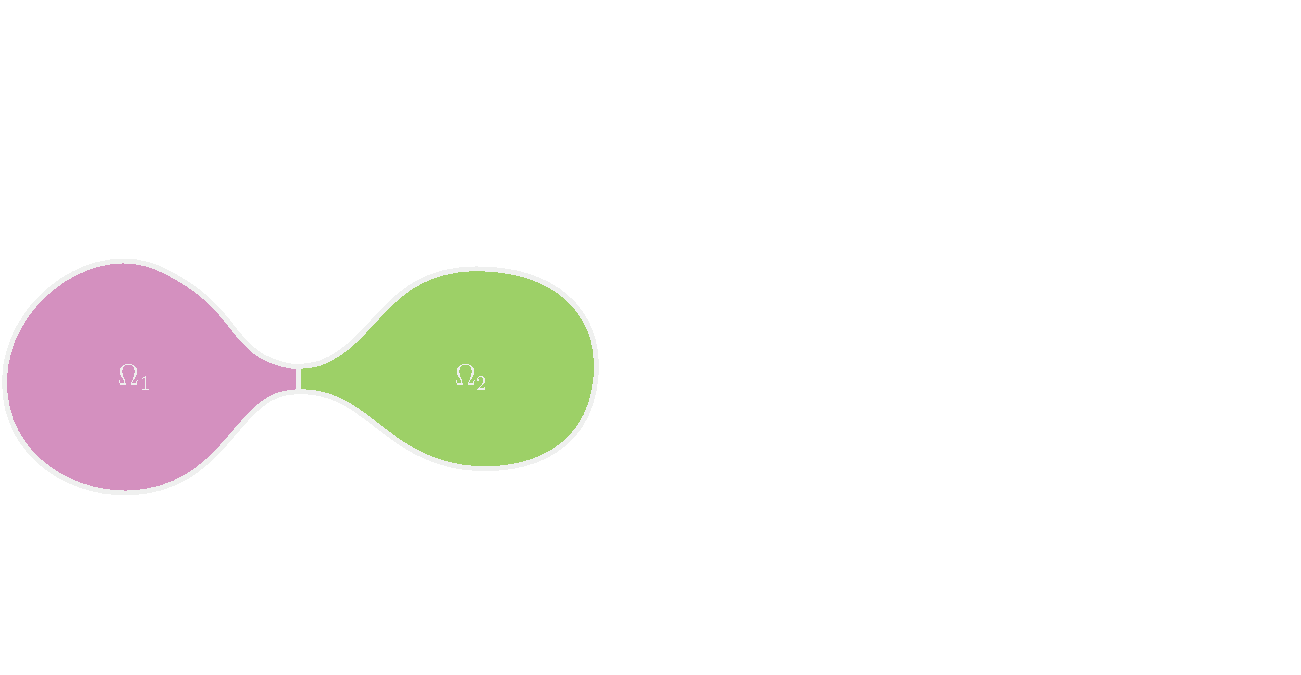
\includegraphics[width=\textwidth]{figures/decomposition1.pdf}}%
\only<3>{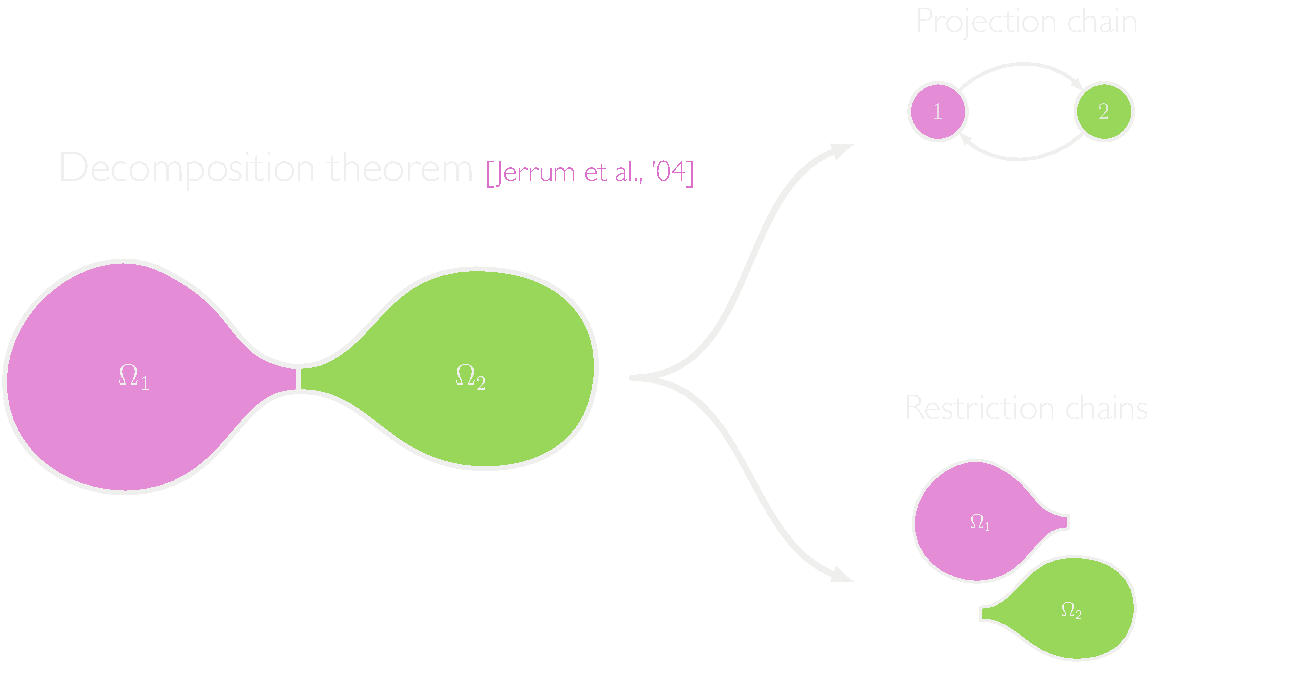
\includegraphics[width=\textwidth]{figures/decomposition2.pdf}}%
\only<4>{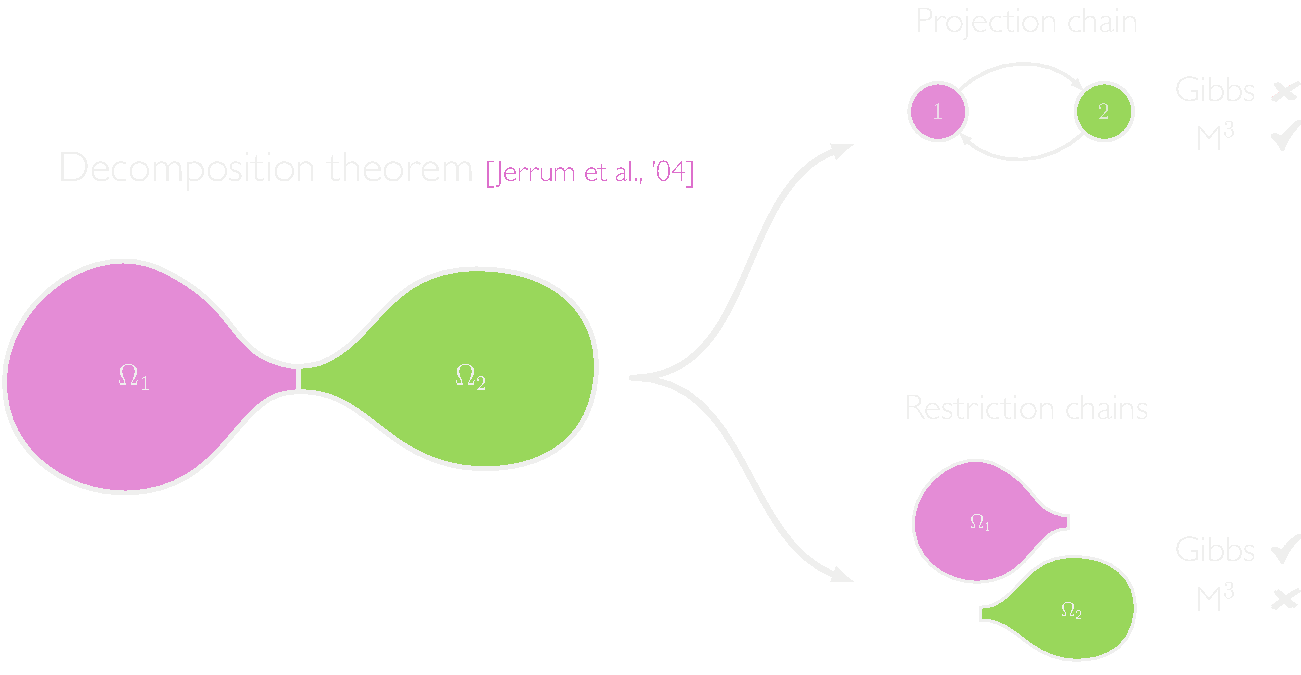
\includegraphics[width=\textwidth]{figures/decomposition.pdf}}%
}
\end{frame}


\begin{frame}{The combined chain}
\vspace{0.5em}
Class of Ising models on the complete graph (Curie-Weiss)

\vspace{1em}
\begin{columns}[t]
\begin{column}{0.3\textwidth}
\centering

\vspace{0.1em}
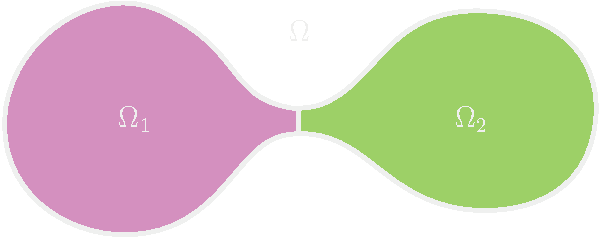
\includegraphics[width=1.2in]{figures/bottleneck1.pdf}

\vspace{2.5em}
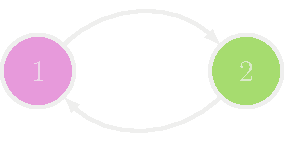
\includegraphics[width=0.8in]{figures/projection.pdf}

\vspace{2em}
\hspace{0.3em}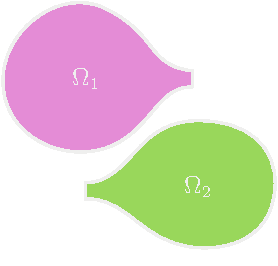
\includegraphics[width=0.9in]{figures/restriction.pdf}
\end{column}

\begin{column}{0.66\textwidth}
\vspace{-1em}
\uncover<2->{%
\begin{itemize}
\small
\item Gibbs $:\ t_{\mathrm{mix}} = \Omega\left( e^{cn} \right)$ \qcitea{Levin et al., '08}
\vspace{0.3em}
\item $\mathrm{M}^3:$\uncover<5>{$\ \ ?$}
\item Combo $:$\uncover<5>{$\ t_{\mathrm{mix}} = \mathcal{O}\left( \displaystyle\frac{n}{\log n}  \right)$ \qciteb{Theorem 2}}
\end{itemize}%
}

\vspace{1.4em}
\begin{itemize}
\item<4-> $\mathrm{M}^3:\ t_{\mathrm{mix}} = \mathcal{O}(1)$ \qciteb{Lemma 1}
\end{itemize}

\vspace{3.2em}
\begin{itemize}
\item<3-> Gibbs $:\ t_{\mathrm{mix}} = \Theta\left( \displaystyle\frac{n}{\log n} \right)$ \qcitea{Ding et al., '09}
\end{itemize}
\end{column}
\end{columns}

\end{frame}


\begin{frame}{Constructing the mixture}
\vspace{0.5em}
\only<1-6>{Construction}\only<7>{{\color{col2}Randomized} construction}\only<8->{{\color{col1}Iterative} construction} of $\ q(\cdot) \propto \sum_{i = 1}^{r} \exp\left(m_i(\cdot) \right)$

\uncover<2->{%
\vspace{2em}
\begin{algorithmic}
  \REQUIRE Set function $F$, mixture size $r$
  \vspace{0.5em}
  \FOR{$i = 1$ \TO $r$}
  \vspace{0.3em}
  \LET{$\sigma$}{\only<1-6>{Permutation of $V$}\only<7>{{\color{col2}Random permutation of $V$}}\only<8->{{\color{col1}\textsc{Greedy}$\Big(F(\cdot) - \log\sum_{j = 1}^{i-1} \exp(m_j(\cdot))\Big)$}}}
  \vspace{0.3em}
  \LET{$m_i$}{\only<1-2>{Modular function that approximates $F$ at $\sigma$}\only<3-6>{\color{col2}\textsc{SemiGradient}$\left(F, \sigma\right)$}\only<7->{\textsc{SemiGradient}($F$, $\sigma$)}}
  \vspace{0.3em}
  \ENDFOR
  \RETURN $\{m_1, \ldots, m_r\}$
\end{algorithmic}%
}

\vspace{2em}
\begin{itemize}
\item<4-> Submodularity $\rightarrow$ natural diminishing returns property
\item<5-> Sub-/supergradients $\rightarrow$ modular lower/upper approx. \qcitea{Iyer et al., '13}
\item<6-> Construction works for general set functions $F$
\end{itemize}
\end{frame}


\begin{frame}{Experiments}
\vspace{1em}
\centering
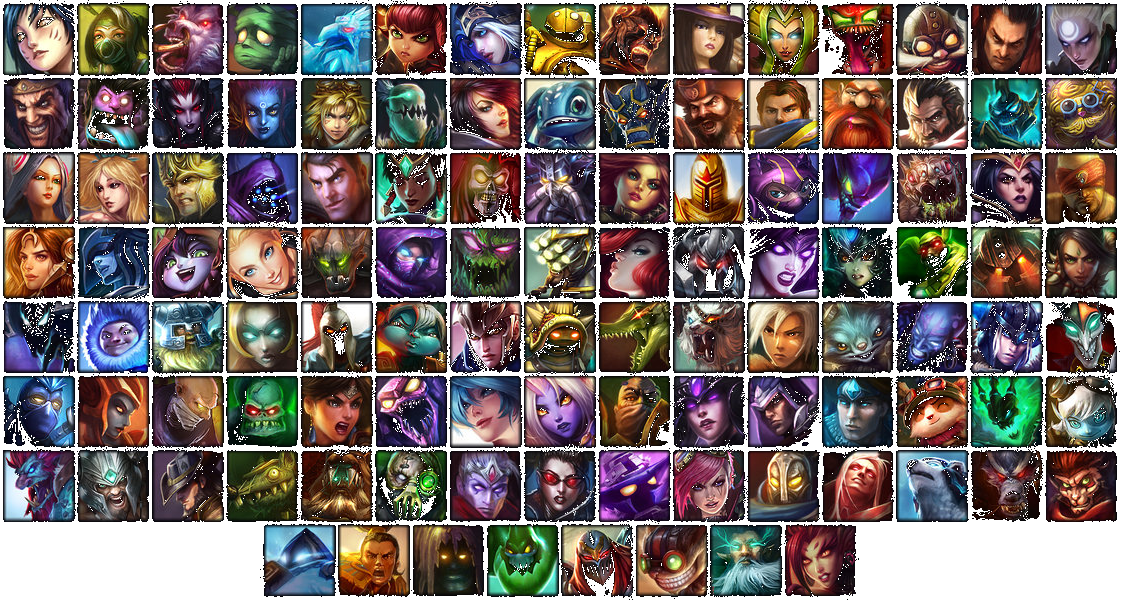
\includegraphics[width=2.3in]{figures/lol_champs.png}

\vspace{1em}
\begin{itemize}
\item<2-> $|V| = 48$
\vspace{0.5em}
\item<3-> 8.5k teams of 5 characters
\vspace{0.5em}
\item<4-> $F$ is a (submodular) facility location diversity model \qcitea{Tschiatschek et al., '16}
\begin{align*}
F(S) = \sum_{i \in S} w_i + \sum_{j=1}^L \max_{i \in S}c_{ij}
\end{align*}
\end{itemize}
\end{frame}


\begin{frame}{Experiments}
\vspace{1em}
\centering
\only<1>{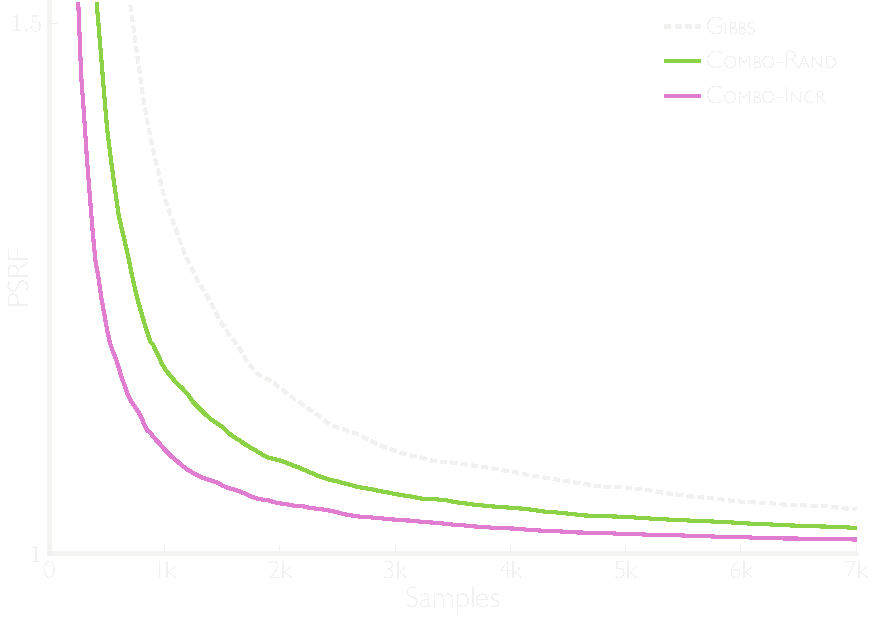
\includegraphics[width=\textwidth,trim=0 0 0 0,clip]{figures/exp1.pdf}}%
%\only<2>{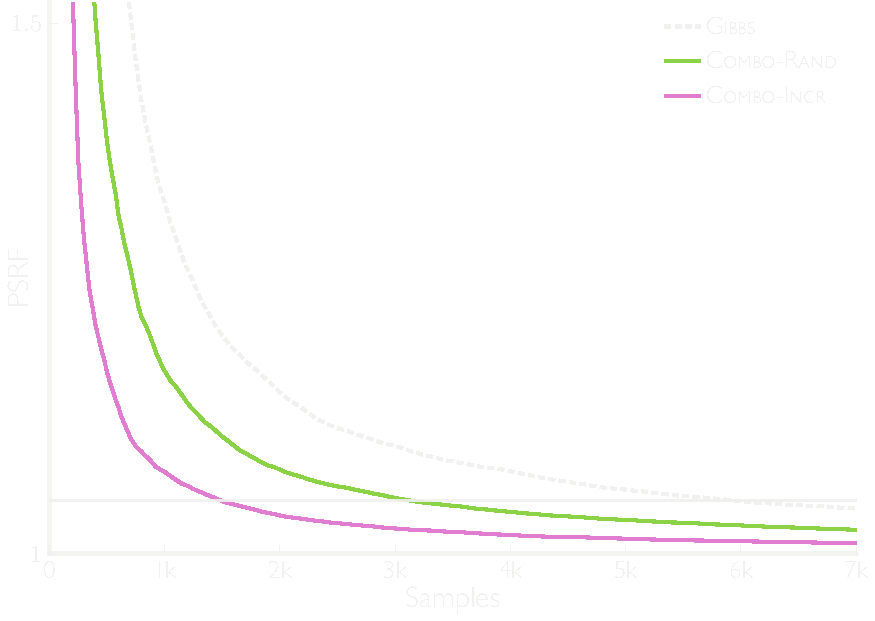
\includegraphics[width=\textwidth,trim=0 0 0 0,clip]{figures/exp1_line.pdf}}%
%\only<3>{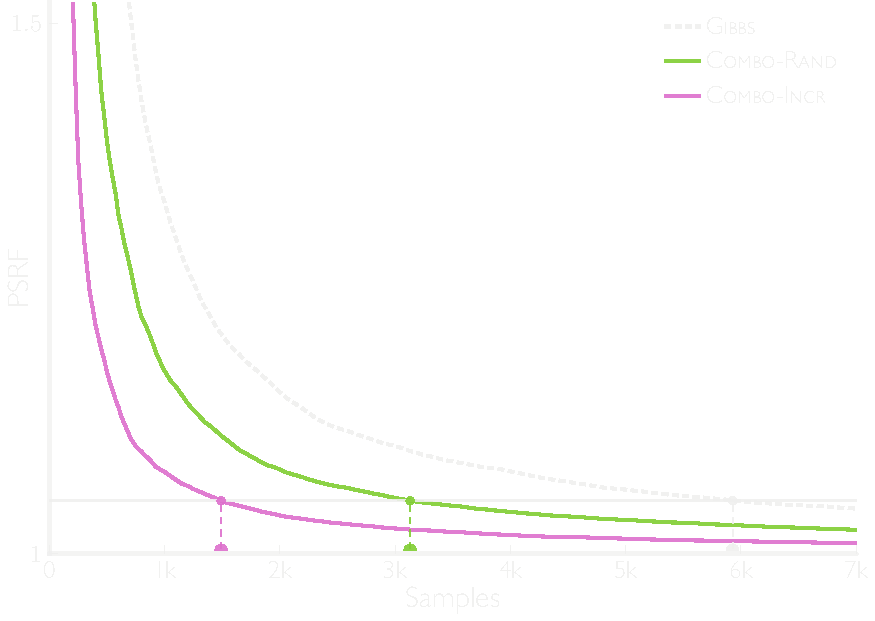
\includegraphics[width=\textwidth,trim=0 0 0 0,clip]{figures/exp1_line_dots.pdf}}%
\end{frame}


\begin{frame}{Experiments}
\vspace{1em}
\centering
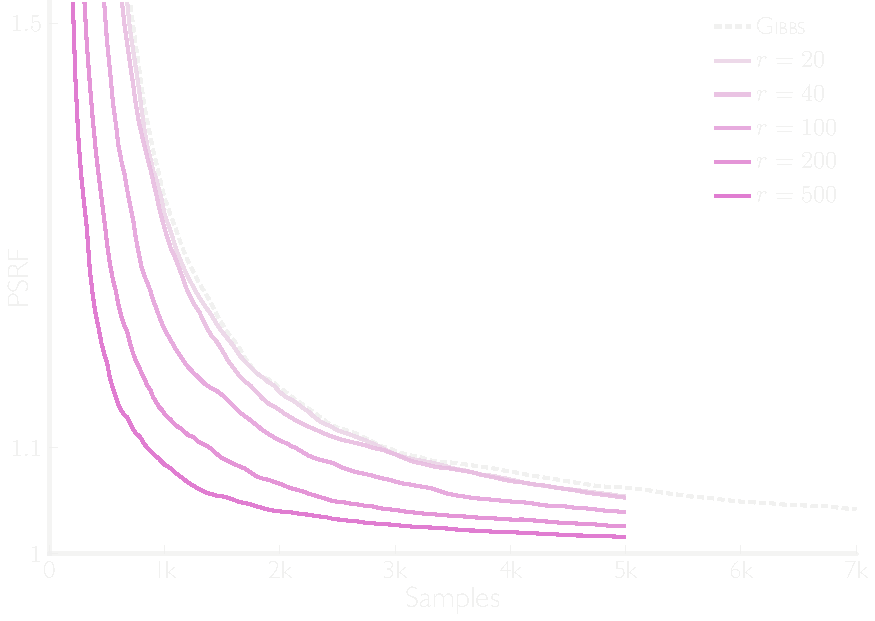
\includegraphics[width=\textwidth,trim=0 0 0 0,clip]{figures/exp2.pdf}
\end{frame}


\begin{frame}{Experiments}
\vspace{1em}
\centering
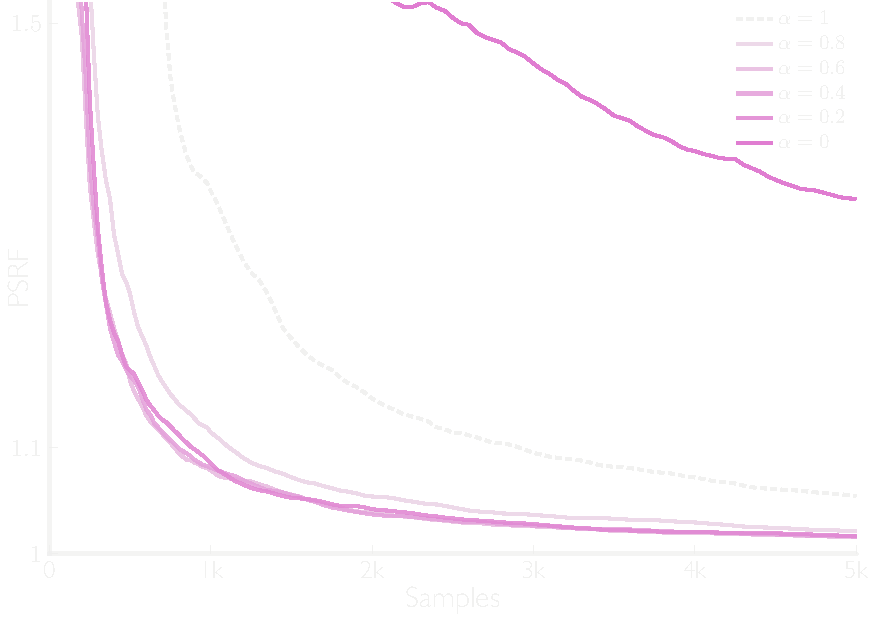
\includegraphics[width=\textwidth,trim=0 0 0 0,clip]{figures/exp3.pdf}
\end{frame}


\begin{frame}{Conclusion}
\vspace{1em}
\centering
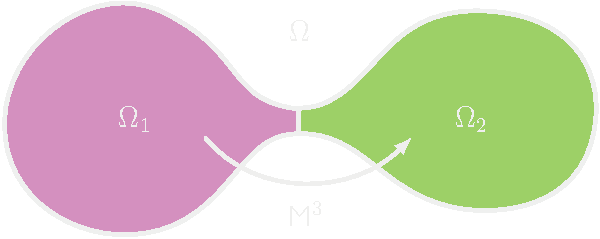
\includegraphics[width=3.5in]{figures/bottleneck_conclusion.pdf}

\vspace{1.5em}
\begin{itemize}
  \item<1-> $\mathrm{M}^3$ sampler $\rightarrow$ propose global moves to overcome bottlenecks
  \vspace{1em}
  \item<2-> Combined sampler $\rightarrow$ analysis based on decomposition theorem
  \vspace{1em}
  \item<3-> Semigradient construction $\rightarrow$ incorporate ideas from optimization
\end{itemize}

\end{frame}

\end{document}
